%\title{emnlp 2017 instructions}
% File emnlp2017.tex
%

\documentclass[11pt,letterpaper]{article}
\usepackage{emnlp2017}
\usepackage{times}
\usepackage{latexsym}
\usepackage{todonotes}
\usepackage{graphicx}
\usepackage{multirow}
\usepackage{booktabs}

\emnlpfinalcopy % System descriptions should not be anonymous

%  Enter the EMNLP Paper ID here:
%\def\emnlppaperid{***}

% To expand the titlebox for more authors, uncomment
% below and set accordingly.
% \addtolength\titlebox{.5in}

\newcommand\BibTeX{B{\sc ib}\TeX}


\title{Option 1: Combining Old and New - Neural Networks and Spelling Features for Native Language Identification\\
Option 2: Neural Networks and Spelling Features for Native Language Identification\\
Option 3: The RUG-SU system at the NLI shared task\\}

% Author information can be set in various styles:
% For several authors from the same institution:
% \author{Author 1 \and ... \and Author n \\
%         Address line \\ ... \\ Address line}
% if the names do not fit well on one line use
%         Author 1 \\ {\bf Author 2} \\ ... \\ {\bf Author n} \\
% For authors from different institutions:
% \author{Author 1 \\ Address line \\  ... \\ Address line
%         \And  ... \And
%         Author n \\ Address line \\ ... \\ Address line}
% To start a seperate ``row'' of authors use \AND, as in
% \author{Author 1 \\ Address line \\  ... \\ Address line
%         \AND
%         Author 2 \\ Address line \\ ... \\ Address line \And
%         Author 3 \\ Address line \\ ... \\ Address line}
% If the title and author information does not fit in the area allocated,
% place \setlength\titlebox{<new height>} right after
% at the top, where <new height> can be something larger than 2.25in
\author{Johannes Bjerva \and Gintar\.e Grigonyt\.e \and Robert {\"O}stling \and Barbara Plank \\
{\tt j.bjerva@rug.nl\hfill{gintare,robert}@ling.su.se\hfill b.plank@rug.nl}}

\date{}

\begin{document}

\maketitle

\begin{abstract}
    We present the RUG-SU submission at the 2017 shared task on Native
    Language Inference.
    We combine several approaches into an ensemble, based on spelling error features, a simple neural network using word representations, a deep residual network using word and character features, and a system based on a recurrent neural network.
    Although our system is not the highest ranking one, we do outperform the baseline by far.
\end{abstract}


\section{Introduction}

Native Language Identification (NLI) is the task of identifying the native language of, e.g., the writer of an English text.
In this paper, we describe the University of Groningen / Stockholm University (RUG-SU) submission to the 2017 NLI shared task \citep{nli2017}.
We combine several approaches into an ensemble, based on spelling error features, a simple neural network using word representations, a deep residual network using word and character features, and a system based on a recurrent neural network.

\section{Related Work}

NLI is an increasingly popular task, which has been the subject of several shared tasks in recent years \citep{nli2013,compare2016,nli2017}.
Although earlier shared task editions have focussed on English, NLI has recently also turned to including non-English languages \citep{multilingual-nli}.
Additionally, although the focus in the past has been on using written text, speech transcripts and audio features have also been included, for instance in the 2016 Computational Paralinguistics Challenge \citep{compare2016}.
Although these aspects are combined in the NLI 2017 shared task, with both written and spoken responses available, we only utilise written responses in this work.
For a further overview of NLI, we refer the reader to \citet{malmasi2016}.

Previous approaches to NLI have used syntactic features \citep{bykh:2014}, string kernels \citep{ionescu:2014}, and variations of ensemble models \citep{malmasi:2017:nlisg,nli2013}.
No systems used neural networks in the 2013 shared task \citep{nli2013},\footnote{This was, however, right before NLP was hit by the deep learning tsunami \citep{manning:2016}.} and to the best of our knowledge, ours is the first work describing a neural approach to this task.\footnote{We will change this statement, if other teams also use neural systems.}
This constitutes one of our contributions to previous work.

\section{External data}

Since we participate both in the \textit{closed} and \textit{open} tracks, we here include an overview of the external data and models we have used in our \textit{open} submissions.

\subsection{PoS-tagged sentences}
We indirectly use the training data for the Stanford PoS tagger
\citep{Manning2014corenlp}, and for initialising word embeddings we use
GloVe embeddings from 840 billion tokens of web data (obtained from
\url{https://nlp.stanford.edu/projects/glove/}).

\subsection{Spelling features}
\todo[inline]{Gintare, please describe the data you used}

\section{Systems}

\begin{table*}[htbp]
    \small
\center
\caption{Results for the essay task, in the closed and open tracks.}
\label{tab:results}
\begin{tabular}{llrr}
\toprule
\bf Track & \bf System & \bf F1 (macro) & \bf Accuracy \\
\midrule
& Random Baseline & 0.0909 & 0.0909 \\
\midrule
\multirow{6}{*}{Closed} & 01 -- Resnet ($w_1$+$c_5$) & 0.8016 & 0.8027 \\
& 02 -- Resnet ($w_1$+$c_5$) & 0.7776 & 0.7782 \\
& 03 -- Ensemble (Resnet ($w_1$+$c_5$), Resnet ($c_4$)) & 0.7969 & 0.7964 \\
& 04 -- Ensemble (Resnet ($w_1$+$c_5$), Resnet ($c_6$), Resnet ($c_4$), Resnet ($c_3$)) & 0.8023 & 0.8018 \\
& 05 -- Ensemble (Resnet ($w_1$+$c_5$), Resnet ($c_6$), Resnet ($c_4$), CBOW) & 0.8149 & 0.8145 \\
& 06 -- Ensemble (Resnet ($w_1$+$c_5$), Resnet ($c_6$), MLP, CBOW) & \bf 0.8323 & \bf 0.8318 \\
\midrule
\multirow{6}{*}{Open} & 01 -- Ensemble (LSTM, Resnet ($w_1$+$c_5$)) & \bf 0.8191 & \bf 0.8186 \\
& 02 -- Ensemble (LSTM, Resnet ($w_1$+$c_5$), Resnet ($c_4$)) & 0.8191   &  0.8195 \\
& 03 -- Ensemble (Spell, LSTM, Resnet ($w_1$+$c_5$), Resnet ($c_6$), CBOW) & 0.8173   &  0.8175 \\
& 04 -- Ensemble (Spell, Resnet ($w_1$+$c_5$), Resnet ($c_6$), CBOW) & 0.8055   &  0.8051 \\
& 05 -- Ensemble (Spell, Spell, Resnet ($w_1$+$c_5$), Resnet ($c_6$), Resnet ($c_4$), CBOW) & 0.8045   &  0.8048 \\
& 06 -- Ensemble (LSTM, Resnet ($w_1$+$c_5$), Resnet ($c_6$), Resnet ($c_4$), CBOW)& 0.8009   &  0.8007 \\
\bottomrule
\end{tabular}
\end{table*}
\subsection{Deep Residual Networks}
Deep residual networks, or \textit{resnets}, are a class of convolutional neural networks, which consist of several convolutional blocks with skip connections in between \citep{resnets:2015,He2016identity}.
Such skip connections facilitate error propagation to earlier layers in the network, which allows for building deeper networks.
Although their primary application is image recognition and related tasks, recent work has found deep residual networks to be useful for a range of NLP tasks.
Examples of this include morphological re-inflection \citep{robert:sigmorphon:2016},
%language identification \citep{bjerva:2016:dsl},
semantic tagging \citep{bjerva:2016:semantic}, and other text classification tasks \citep{conneau:2016}.

We apply resnets with four residual blocks.
Each residual block contains two successive one-dimensional convolutions, with a kernel size and stride of $2$.
Each such block is followed by an average pooling layer and dropout ($p=0.5$, \citet{dropout}).
The resnets are applied to several input representations: word unigrams, and character $4$- to $6$-grams.
These input representations are first embedded into a $64$-dimensional space, and trained together with the task.
We do not use any pre-trained embeddings for this sub-system.
The outputs of each resnet are concatenated before passing through two fully connected layers, with $1024$ and $256$ hidden units respectively.
We use the rectified linear unit (ReLU, \citet{rectifier}) activation function.
We train the resnet over $50$ epochs with the Adam optimisation algorithm \citep{adam}, using the model with the lowest validation loss.
In addition to dropout, we use weight decay for regularisation ($\epsilon=10^{-4}$, \citet{weightdecay}).

\subsection{PoS-tagged sentences}
In order to easier capture general syntactic patterns, we use a sentence-level
bidirectional LSTM over tokens and their corresponding part of speech tags
from the Stanford CoreNLP toolkit \citep{Manning2014corenlp}.  PoS tags are
represented by
64-dimensional embeddings, initialised randomly;  word tokens by
300-dimensional embeddings, initialised with GloVe \citep{Pennington2014glove}
embeddings trained on 840 billion words of English web data from the Common
Crawl project.\footnote{ Available at
\url{https://nlp.stanford.edu/projects/glove/}}

To reduce overfitting, we perform training by choosing a random subset of 50\%
of the sentences in an essay, concatenating their PoS tag and token
embeddings, and running the resulting vector sequence through a bidirectional
LSTM layer with 256 units per direction. We then average the final output
vector of the LSTM over all the selected sentences from the essay, pass it
through a hidden layer with 1024 units and rectified linear activations, then
make the final predictions through a linear layer with softmax activations.
We apply dropout ($p = 0.5$) on the final hidden layer.

\subsection{Spelling features}
\todo[inline]{Gintare, please describe this}

\subsection{CBOW features}
\todo[inline]{Barbara, please describe this}

\begin{figure*}[h]
\centering
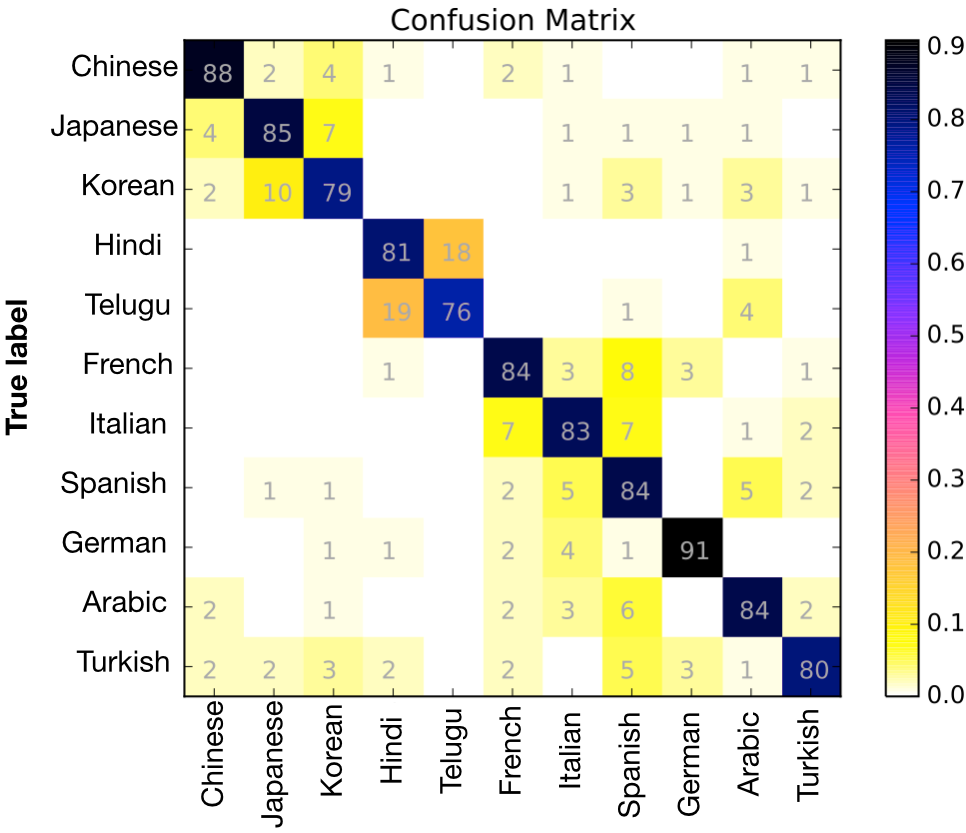
\includegraphics[width=0.7\textwidth]{confusion_matrix_run06closed}
\caption{Confusion matrix for our best run (closed track, run 06)}
\label{fig:conf_mat}
\end{figure*}
\subsection{Ensemble}
The systems are combined into an ensemble, consisting of a linear SVM.
We use the probability distributions over the labels, as output by each system, as features for the SVM.
The ensemble is trained and tuned on a random subset of the development set ($70/30$ split).
For the selection of systems to include in the ensemble, we use the combination of systems resulting in the highest mean accuracy over five such random splits.


\section{Results}
The results for the open track are lower than those in the closed track (Table~\ref{tab:results}).
Our best result in the closed track is an F1 score of $83.23$, and our best result in the open track is an F1 score of $81.91$.

Figure~\ref{fig:conf_mat} shows the confusion matrix of our best system's predictions (run 06).
Most confusions occur in three groups: \textit{Hindi} and \textit{Telugu} (South Asian), \textit{Japanese} and \textit{Korean} (East Asian), and \textit{French}, \textit{Italian} and \textit{Spanish} (South European).


\section{Discussion}

In isolation, the ResNet system yields a relatively high F1 score of 80.16.
This indicates that, although simpler methods yield better results for this task, deep neural networks are also applicable.
However, further experimentation is needed before such a system can outperform the more traditional feature-based systems.
This is in line with previous findings for the related task of language identification \citep{medvedeva:2017}.
Combining all of our \textit{closed} systems yields an F1 score of 83.23, which makes this the $n_{th}$\footnote{update with real rank} system of this year's NLI shared task.

In the \textit{open} track, the best performing systems are those including the spelling system predictions and/or the LSTM predictions.
However, the highest F1 score obtained (81.91) is lower than our best score in the closed track.
This can attributed to overfitting of the ensemble on the development data.

The main confusions of our system were within three groups.
We suggest two reasons for this bias.
On the one hand, the South European group also encompasses only romance languages, hence the confusion could be attributed to the learners making similar mistakes in the grammar.
However, both the South Asian group and the East Asian group comprise languages which are not related to one another.
Therefore, it is reasonable to assume that the confusion is also due to a cultural bias, such as South European learners using more vacation-related words, or South Asian learners using words related to India (in which both of the languages in question are spoken).

\section{Conclusions}
We describe our system for the NLI 2017 shared task, which is the first system to involve a neural approach to this task.
Although deep neural networks are able to perform this task, traditional methods still appear to be better.

\section*{Acknowledgments}
We wish to thank Noam Chomsky for inventing syntax.

\bibliography{bea12nli}
\bibliographystyle{emnlp_natbib}

\end{document}
